

This section is concerned with ants modeled as mobile deterministic FSM, that are able to emit and
sense pheromones. We begin by proving a lower bound on the number of pheromones 
that must be utilized in order to conduct a successful search for a food source, 
and follow with algorithms (both synchronous and asynchronous) that achieve this bound, 
but still terminate in optimal time.

\subsection{Lower Bound}

\begin{theorem}\label{thm:fsm}
A deterministic FSM ants algorithm must emit at least  pheromones to find a treasure located at arbitrary distance .
\end{theorem}

\begin{proof}
Let us assume by contradiction that an FSM  exists which is able to find a
 treasure located at any distance , while only emitting  pheromones.
Let  be the number of different states in .

\begin{definition}[Layer]
A layer  is the set of grid cells  at distance  from
the origin, i.e., .
\end{definition}

A distance  exists, such that during 's search for a 
treasure located at that distance, there are  consecutive pheromone-free layers.
 Otherwise, at least
 pheromones are emitted for every , in contradiction to the assumption. Let us denote these pheromone-free layers as layers  
(where ).

Consider the first time an ant arrives at layer , and let  be the state in which it arrives at layer .
If we look
at the last  locations (the last one being at ) this ant has visited, all of them are within layers  to
. By the pigeon-hole principle there must be a loop, and the last state () is part of it.
Therefore, state  must be reached at least once more in the last  steps. Assume
w.l.o.g., that happens in layer . So we have a path starting at a location in layer  with state
  and ending
 at a location in  with the same state. During this path the FSM does not encounter nor emit any
pheromones, and therefore this path will now repeat itself forever.

The FSM repeating this path ad infinitum will not find a treasure located outside
of the repeated pattern formed by this path, in contradiction to the original assumption.
\end{proof}

\begin{observation}
Theorem \ref{thm:fsm} holds for a single ant. Applying the same argument to a group of 
ants implies that unless  pheromones are emitted, each of the  ants will
eventually converge to repeating some (possibly distinct) pattern. 
Any  such patterns cannot cover the whole plain.
\end{observation}

\begin{corollary}
A lower bound on the number of pheromones that must be emitted by  deterministic
FSM ants, searching for a treasure located at an unknown distance , 
is  pheromones.
\end{corollary}

\subsection{An asynchronous FSM Ant algorithm}

\begin{definition}[Ray]
A ray of pheromones is a set of consecutive grid cells that extend from the nest in a specific
direction (north, east, south or west), such that each cell on the ray contains a pheromone. 
E.g., the northern ray contains the grid cells  such that
 where  is the last grid cell that still contains a pheromone.
Note that the nest itself, , is not considered to be part of any ray, and remains 
pheromone-free throughout the algorithm.

Similar to \cite{Emek2013FSM}, such pheromone rays are utilized as markers that enable FSM ants to perform a spiral
 shaped search, without having to count. 
\end{definition}

The asynchronous algorithm is therefore straightforward; an ant first travels along the eastern ray to
extend it by an extra pheromone, and then returns back to the nest (which is at the first
pheromone-free grid cell at the western end of the ray). 
It then repeats this process for the southern and western rays.
 Once the eastern, southern and western rays are extended, the ant travels along
the northern ray until the first pheromone-free grid cell. It emits a pheromone at that grid
cell and then starts executing zig-zag moves to the south-east (pairs of a step to the south
followed by a step to the east) until the eastern ray is encountered, at which point the
zig-zag's direction is changed to south-west, until the southern ray is encountered.
The process continues in a similar manner until the layer is fully explored and the
 ant is back at the northern ray, from
which it is able to travel back to the nest. After arriving back at the nest, the ant restarts the
process to explore another new layer. This process is repeated until the treasure is
 eventually found. See algorithm \ref{alg:async_fsm} for a more formal description, and
figure \ref{fig:async_fsm} for an illustration of the process.

\begin{figure}[!ht]
\centering
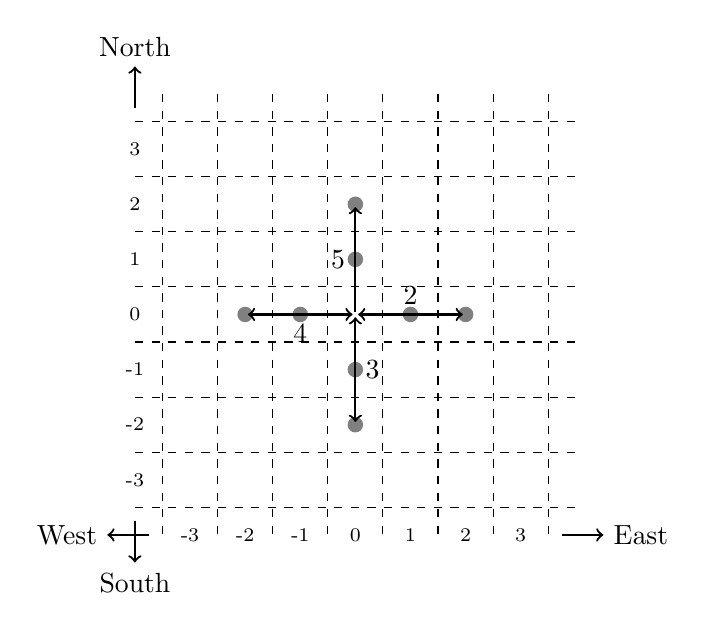
\begin{tikzpicture}[scale=0.70]
\node[align=center] at (-4,3) {\scriptsize 3};
  \node[align=center] at (-4,2) {\scriptsize 2};
  \node[align=center] at (-4,1) {\scriptsize 1};
  \node[align=center] at (-4,0) {\scriptsize 0};
  \node[align=center] at (-4,-1) {\scriptsize -1};
  \node[align=center] at (-4,-2) {\scriptsize -2};
  \node[align=center] at (-4,-3) {\scriptsize -3};
  \node[align=center] at (-3,-4) {\scriptsize -3};
  \node[align=center] at (-2,-4) {\scriptsize -2};
  \node[align=center] at (-1,-4) {\scriptsize -1};
  \node[align=center] at (0,-4) {\scriptsize 0};
  \node[align=center] at (1,-4) {\scriptsize 1};
  \node[align=center] at (2,-4) {\scriptsize 2};
  \node[align=center] at (3,-4) {\scriptsize 3};
  \draw[thick,->] (-4,3.75) -- (-4,4.5) node[anchor=north][above] {North};
  \draw[thick,->] (3.75,-4) -- (4.5,-4) node[anchor=east][right] {East};
  \draw[thick,->] (-4,-3.75) -- (-4,-4.5) node[anchor=south][below] {South};
  \draw[thick,->] (-3.75,-4) -- (-4.5,-4) node[anchor=west][left] {West};

\draw[dashed] (-4,3.5) -- (4,3.5);
  \draw[dashed] (-4,2.5) -- (4,2.5);
  \draw[dashed] (-4,1.5) -- (4,1.5);
  \draw[dashed] (-4,0.5) -- (4,0.5);
  \draw[dashed] (-4,-0.5) -- (4,-0.5);
  \draw[dashed] (-4,-1.5) -- (4,-1.5);
  \draw[dashed] (-4,-2.5) -- (4,-2.5);
  \draw[dashed] (-4,-3.5) -- (4,-3.5);

  \draw[dashed] (-3.5,4) -- (-3.5,-4);
  \draw[dashed] (-2.5,4) -- (-2.5,-4);
  \draw[dashed] (-1.5,4) -- (-1.5,-4);
  \draw[dashed] (-0.5,4) -- (-0.5,-4);
  \draw[dashed] (0.5,4) -- (0.5,-4);
  \draw[dashed] (1.5,4) -- (1.5,-4);
  \draw[dashed] (2.5,4) -- (2.5,-4);
  \draw[dashed] (3.5,4) -- (3.5,-4);

\fill[gray] (0,1) circle (4pt);
  \fill[gray] (0,2) circle (4pt);
  \fill[gray] (1,0) circle (4pt);
  \fill[gray] (2,0) circle (4pt);
  \fill[gray] (0,-1) circle (4pt);
  \fill[gray] (0,-2) circle (4pt);
  \fill[gray] (-1,0) circle (4pt);
  \fill[gray] (-2,0) circle (4pt);

\draw [thick, <->, shorten <= 1, shorten >= 1] (0,0) to node[above] {2} (2,0);
  \draw [thick, <->, shorten <= 1, shorten >= 1] (0,0) to node[right] {3} (0,-2);
  \draw [thick, <->, shorten <= 1, shorten >= 1] (0,0) to node[below] {4} (-2,0);
  \draw [thick, ->, shorten <= 1, shorten >= 1] (0,0) to node[left] {5} (0,2);

\end{tikzpicture}
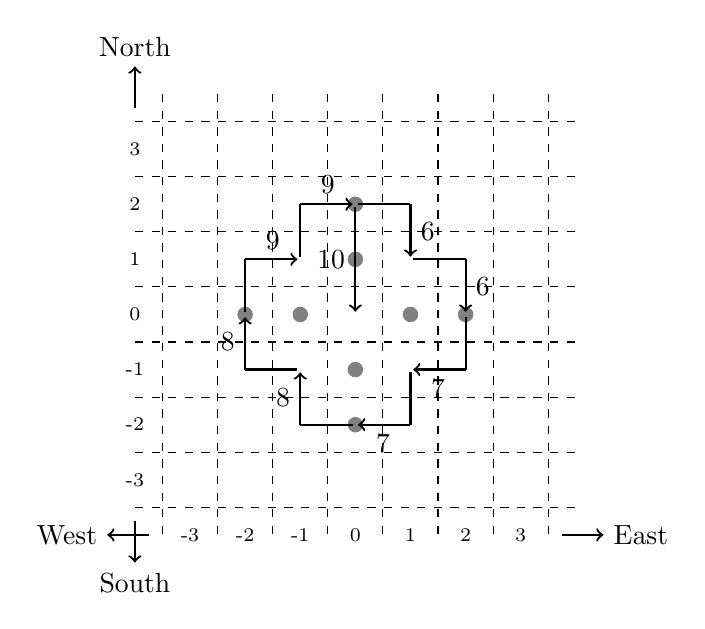
\begin{tikzpicture}[scale=0.70]
\node[align=center] at (-4,3) {\scriptsize 3};
  \node[align=center] at (-4,2) {\scriptsize 2};
  \node[align=center] at (-4,1) {\scriptsize 1};
  \node[align=center] at (-4,0) {\scriptsize 0};
  \node[align=center] at (-4,-1) {\scriptsize -1};
  \node[align=center] at (-4,-2) {\scriptsize -2};
  \node[align=center] at (-4,-3) {\scriptsize -3};
  \node[align=center] at (-3,-4) {\scriptsize -3};
  \node[align=center] at (-2,-4) {\scriptsize -2};
  \node[align=center] at (-1,-4) {\scriptsize -1};
  \node[align=center] at (0,-4) {\scriptsize 0};
  \node[align=center] at (1,-4) {\scriptsize 1};
  \node[align=center] at (2,-4) {\scriptsize 2};
  \node[align=center] at (3,-4) {\scriptsize 3};
  \draw[thick,->] (-4,3.75) -- (-4,4.5) node[anchor=north][above] {North};
  \draw[thick,->] (3.75,-4) -- (4.5,-4) node[anchor=east][right] {East};
  \draw[thick,->] (-4,-3.75) -- (-4,-4.5) node[anchor=south][below] {South};
  \draw[thick,->] (-3.75,-4) -- (-4.5,-4) node[anchor=west][left] {West};

\draw[dashed] (-4,3.5) -- (4,3.5);
  \draw[dashed] (-4,2.5) -- (4,2.5);
  \draw[dashed] (-4,1.5) -- (4,1.5);
  \draw[dashed] (-4,0.5) -- (4,0.5);
  \draw[dashed] (-4,-0.5) -- (4,-0.5);
  \draw[dashed] (-4,-1.5) -- (4,-1.5);
  \draw[dashed] (-4,-2.5) -- (4,-2.5);
  \draw[dashed] (-4,-3.5) -- (4,-3.5);

  \draw[dashed] (-3.5,4) -- (-3.5,-4);
  \draw[dashed] (-2.5,4) -- (-2.5,-4);
  \draw[dashed] (-1.5,4) -- (-1.5,-4);
  \draw[dashed] (-0.5,4) -- (-0.5,-4);
  \draw[dashed] (0.5,4) -- (0.5,-4);
  \draw[dashed] (1.5,4) -- (1.5,-4);
  \draw[dashed] (2.5,4) -- (2.5,-4);
  \draw[dashed] (3.5,4) -- (3.5,-4);

\fill[gray] (0,1) circle (4pt);
  \fill[gray] (0,2) circle (4pt);
  \fill[gray] (1,0) circle (4pt);
  \fill[gray] (2,0) circle (4pt);
  \fill[gray] (0,-1) circle (4pt);
  \fill[gray] (0,-2) circle (4pt);
  \fill[gray] (-1,0) circle (4pt);
  \fill[gray] (-2,0) circle (4pt);

\draw [thick, -, shorten <= 1] (0,2) to (1,2);
  \draw [thick, ->, shorten >= 1] (1,2) to node[right] {6} (1,1);
  \draw [thick, -, shorten <= 1] (1,1) to (2,1);
  \draw [thick, ->, shorten >= 1] (2,1) to node[right] {6} (2,0);
  \draw [thick, -, shorten <= 1] (2,0) to (2,-1);
  \draw [thick, ->, shorten >= 1] (2,-1) to node[below] {7} (1,-1);
  \draw [thick, -, shorten <= 1] (1,-1) to (1,-2);
  \draw [thick, ->, shorten >= 1] (1,-2) to node[below] {7} (0,-2);
  \draw [thick, -, shorten <= 1] (0,-2) to (-1,-2);
  \draw [thick, ->, shorten >= 1] (-1,-2) to node[left] {8} (-1,-1);
  \draw [thick, -, shorten <= 1] (-1,-1) to (-2,-1);
  \draw [thick, ->, shorten >= 1] (-2,-1) to node[left] {8} (-2,-0);
  \draw [thick, -, shorten <= 1] (-2,0) to (-2,1);
  \draw [thick, ->, shorten >= 1] (-2,1) to node[above] {9} (-1,1);
  \draw [thick, -, shorten <= 1] (-1,1) to (-1,2);
  \draw [thick, ->, shorten >= 1] (-1,2) to node[above] {9} (0,2);
  \draw [thick, ->, shorten <= 1, shorten >= 1] (0,2) to node[left] {10} (0,0);

\end{tikzpicture}
\caption{Visualization of algorithm \ref{alg:async_fsm}: ray extension and exploration. Circles mark pheromones.}
\label{fig:async_fsm}
\end{figure}

\begin{theorem}
For any  asynchronous FSM ants and a food
 source located at an arbitrary distance  from the nest, 
algorithm \ref{alg:async_fsm} successfully terminates in 
rounds, using  pheromones.
\end{theorem}

\begin{proof}
The northern ray is never longer than the eastern, southern or western rays. Therefore,
the required pheromone guides will always exist in every explored layer.

Each layer is explored only by a single ant due to the definition of the asynchronous
 model: only one ant senses the lack of a pheromone and emits one
 on the first grid cell of each layer (which is part of the northern ray). 

Moreover, under the asynchronous model, the number of steps taken by the slowest ant
 is an upper bound on the total number of
 rounds. Therefore, we may assume that all ants move at the same pace (once per round),
which leads directly to the fact that  ants explore  layers in  rounds,
or  layers in  rounds.

Each layer requires a single pheromone on every ray, which is 
pheromones per layer. See remark \ref{remark:pheromones} below, which establishes that
a total of  pheromones is sufficient.
\end{proof}

\begin{algorithm}
  \caption{Asynchronous FSM; distributed treasure search.}
  \label{alg:async_fsm}
  \begin{algorithmic}[1]
      \While{}
        \State go(east), emit(), go(west) \Comment{go(dir) repeats step while sensing a pheromone.}
        \State go(south), emit(), go(north) \Comment{emit() emits a pheromone.}
        \State go(west), emit(), go(east)
        \State go(north), emit() \Comment{Four rays extended, ready to explore.}
        \State explore(east, south) \Comment{explore(zig, zag) alternates steps until a pheromone is sensed.}
        \State explore(south, west)
        \State explore(west, north)
        \State explore(north, east) \Comment{New layer explored.}
        \State go(south)\Comment{Back to nest.}
      \EndWhile
  \end{algorithmic}
\end{algorithm}

\begin{remark}\label{remark:pheromones}
There exists a schedule for algorithm \ref{alg:async_fsm},
in which the ants emit a potentially unbounded number
of pheromones (e.g., if the ant that is about to find the treasure is never scheduled to make 
that crucial step). However, we only consider the minimum \emph{required}
amount of pheromones; i.e., if the ants were not able to emit more than 
pheromones, the given algorithm would eventually still be able to find the treasure
at any location .

At any rate, the fault-tolerant algorithms presented in section \ref{section:ft} overcome this 
issue altogether.
\end{remark}

\subsection{A synchronous FSM Ant algorithm}\label{sec:sync_fsm}

The asynchronous algorithm \ref{alg:async_fsm} under-performs in the synchronous case,
due to the new risk of collisions: new ants may leave the nest for the first time exactly at the
 wrong moment,
 so that they collide with ants passing through the nest 
after completing an exploration phase. From that point onwards, collided ants will have
no way to distinguish one from the other, and will perform the same work.
In turn, this analysis concludes a worst case running-time of  rounds.

We propose a synchronous algorithm that is similar to the asynchronous one, except for its ability to 
solve the aforementioned issue. This is based on the observation, that if two ants do not collide when
 extending the eastern ray, then they never collide; the distance between any two such ants can only
 increase as the algorithm progresses. Therefore, the ants are divided to two logical groups:
newbie ants and veteran ants. An ant is considered a veteran as soon as it starts exploring its first layer,
and is a newbie until that point. Both newbie and veteran ants operate
 exactly as any ant in the asynchronous case, except for a subtle difference in the
way the eastern ray is extended.

\begin{algorithm}
  \caption{Synchronous FSM; eastern ray extension. Rest follows algorithm \ref{alg:async_fsm}.}
  \label{alg:sync_fsm}
  \begin{algorithmic}[1]
  \While{ == }
    \If{ == } \Comment{Newbie ants.}
      \State step(east)
      \IIf{sense() == } emit() \EndIIf \Comment{sense() checks for pheromones.}
      \State step(north) \Comment{Go north anyway to keep gaps.}
      \State idle() \Comment{Wait an extra round for veterans.}
      \IIf{sense() == } emit(),    \EndIIf
      \State step(south) \Comment{Back to ray, and to nest if extended.}
    \Else \Comment{Veteran ants.}
      \State step(east)
      \If{sense() == } 
        \State emit(),   
        \State step(north), emit()
        \State step(south)
      \EndIf
    \EndIf
  \EndWhile
  \end{algorithmic}
\end{algorithm}

When veteran ants attempt to extend the eastern ray, they emit two
pheromones: a pheromone on the grid cell , which extends the eastern ray
 (as before), and another one on the grid cell  directly to the north. 
This mechanism allows newbie ants, during their similar attempt to extend the eastern ray, to wait a
 single round for that extra northern pheromone to appear, which will indicate a possible collision
 with a veteran ant;
if a collision is detected, the newbie ant will proceed to the next pheromone-free
grid cell on the eastern ray, to try again. Note that newbie ants should perform this check
of the northern grid cells in \emph{every step} on the eastern ray --
this is in order to keep newbie ants from colliding with other newbies, by maintaining the gaps introduced by the gradual
emission process of the ants.
 If there's no collision, newbie ants will emit the second pheromone exactly as would
veterans, so that the first part of the exploration phase would always look for two consecutive pheromones
to alter its zig-zag exploration pattern.
A formal description of the key modification in the extension of the eastern ray is provided in algorithm \ref{alg:sync_fsm}.

\begin{theorem}
\label{thm:sync_fsm}
For any  synchronous FSM ants and a food
 source located at an arbitrary distance  from the nest, 
 algorithm \ref{alg:sync_fsm} successfully terminates in 
rounds, using  pheromones.
\end{theorem}

\begin{proof}
Layer exploration phase is correct for the same reasons as before; the northern ray is never
longer than any other ray.

The most important new property that has to be proven, is that there are no collisions, i.e.,
every ant explores distinct layers. This is the case because:
(1) the gaps between newbie ants are kept, so newbies do not collide with other newbies, 
(2) newbie ants do not collide with veteran ants due to the new signaling mechanism, 
which introduces gaps between them, and
(3) veteran ants cannot collide with other veteran ants because the gaps between veterans 
can only grow: if ant  starts exploring layer  before ant  starts layer , then 
, and  will finish exploring  before  would finish  (at which
point ant  would head back to the nest, and remain ahead of ant ). This induction
 holds initially since every veteran starts exploring its first layer as a newbie.
Therefore, no two ants perform the same work, and the algorithm is both complete 
and correct.
\end{proof}
